\subsection{Secondary DT Neutrons}

    As of the writing of this thesis, the NIF has four high precision neutron time-of-flight (nToF) detectors that are capable of measuring secondary DT neutron yields. The nTOF detectors work by measuring the time it takes for a neutron to arrive from a source to the detector (the time-of-flight). The energy of the neutron can be related to the arrival time $t$, by the simple equation:
    %
    \begin{equation}
        E_n = \frac{m_n}{2} \left(\frac{d}{t-\tau_B}\right)^2
    \end{equation}
    %
    where $m_n$ is the mass of a neutron, $d$ is the distance between the source and the detector, and $\tau_B$ is the birth time of the neutron. 
    
    The actual neutron detector is a fast organic scintillator who's light goes on to be detected by four photo-detectors (either Photomultiplier Tubes (PMT) or Photodiodes (PD)). The data from each photo-detector is then digitized by a four-channel high bandwith oscilloscope. The channels are all set to different sensitivities so as to increase the dynamic range of the detection system. This is very important for resolving the secondary DT neutron signals which are of order 100 times lower than the primary DD neutron signal levels. All in all, this means there are a total of four scintillators, 16 photo-detectors, and 64 different oscilloscope channels. An example measurement is shown in Figure \ref{fig:ntofExample}.
    
    \begin{figure}[!h]
        \centering
        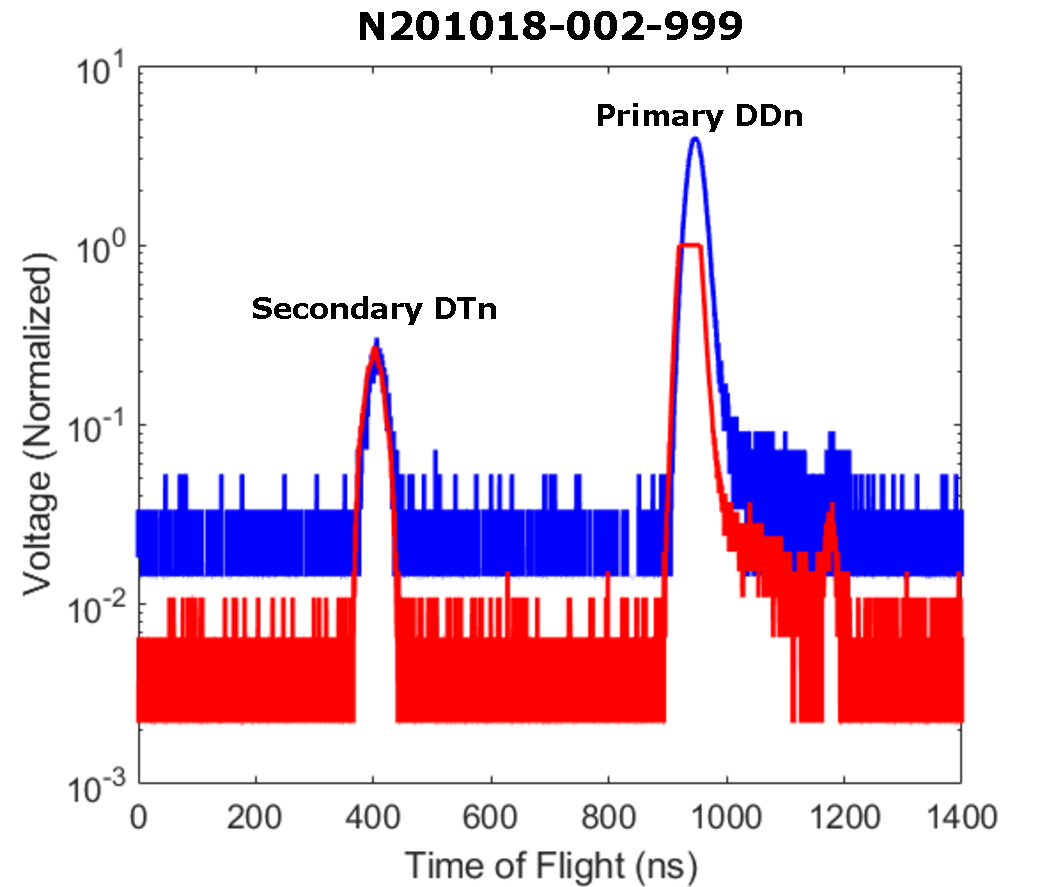
\includegraphics[scale=0.7]{Figures/ntofExample.pdf}
        \caption[Example nTof Traces]{Example data taken from the equatorial NTOF line of sight (SPEC-E) on NIF shot number N201018-002-999. Data in red comes from detector 1 channel 1 and the data in blue comes from detector 3 channel 3. The different detector/channel pairs have different sensitivities and thus different noise floors. }
        \label{fig:ntofExample}
    \end{figure}
    
    As can be seen in Figure \ref{fig:ntofExample} the secondary DT neutrons come much earlier in time than the primary DD neutrons due to their higher energies. This is fortunate because it means the background for the secondary DT neutron measurement is very low. Note also the use of the two different detectors/channels. The channel plotted in red, is significantly more sensitive than the one plotted in blue meaning it can more accurately resolve the secondary DT neutrons. However, this increased sensitivity causes the detector to clip compromising the primary DD neutron signal.  
    
    As stated there are four unique line of sights currently available on the NIF. Their names and exact locations are shown in Table \ref{tab:ntofLocations}.
    
    \begin{table}[!h]
        \centering
        \tabulinesep = 3mm
        \begin{tabu}{c|c c c c}
            Name & SPEC-SP & SPEC-A & SPEC-E & SPEC-NP \\\hline
            Distance (m) & 17.98 & 22.22 & 20.09 & 21.61  \\
            Polar Angle (deg) & 161 & 116 & 90 & 18 \\
            Azimuth Angle (deg) & 56 & 316 & 174 & 303
        \end{tabu}
        \caption[nToF Locations]{Locations of the four nToFs on the NIF capable of meassuring secondary DT neutrons.}
        \label{tab:ntofLocations}
    \end{table}
    
    Calculating the yield from the data is simply a matter of integrating the total charge and multiplying by a calibration constant. Specifically:
    %
    \begin{equation}
        Y_{DTn} = c\times Q
    \end{equation}
    %
    where $c$ is a calibration constant and $Q$ is the total integrated charge given by:
    %
    \begin{equation}
        Q = \frac{\Delta t}{R}\sum_{i} \left(V(i) - V_{BG}\right) 
    \end{equation}
    %
    where $\Delta t$ is the time width of a bin (unusually 0.1 ns), $R$ is the detector's resistance (50 $\Omega$ for every system), $V(i)$ is the voltage in some time bin $i$ that contains signal, and $V_{BG}$ is the average voltage reading in the non-signal region. We calculate the absolute uncertainty on the yield as:
    
    \begin{equation}
        \delta Y = Y * \sqrt{\left(\frac{\delta c}{c}\right)^2 + \left(\frac{\delta Q}{Q}\right)^2 + \left(\frac{\delta N_n}{N_n}\right)^2} 
    \end{equation}
    %
    where $\delta c$ is the uncertainty on the calibration coefficient, $\delta Q$ is the uncertainty in the integrated charge given by:
    %
    \begin{equation}
        \delta Q = \frac{\Delta t}{R} \sigma_V N_{bins}
    \end{equation}
    %
    where $\sigma_V$ is the standard deviation of the voltage in the non-signal region (the noise), and $N_{bins}$ is the number of time bins that contain signal. $N_n$ is the number of neutrons physically detected by the scintillator which is given by:
    %
    \begin{equation}
        N_n = Y \times \left(\frac{1}{4\pi d^2}\right)\times\left(\pi r^2\right) \times n\sigma t
    \end{equation}
    %
    where $r$ is the radius of the scintillator, $n$ is the number density, $\sigma$ is the neutron elastic scattering cross section, and $t$ is the thickness of the scintillator. Finally, $\delta N_n$ is simply the uncertainty on the number of neutrons detected which is simply:
    %
    \begin{equation}
        \delta N_n = \sqrt{N_n}
    \end{equation}
    %
    Various scintillator characteristics used for these calculations are listed in Table \ref{tab:scintCharacteristics}.
    
    \begin{table}[h!]
        \centering
        \tabulinesep = 3mm
        \begin{tabu}{c|c}
            Characteristic  &   Value \\\hline
            Material & Bibenzyl (C$_6$H$_5$CH$_2$)$_2$ \\
            Radius (cm) &  4.16 \\
            Thickness (cm) & 5.04 \\
            Mass Density (g/cc) & 0.978 \\
            Cross Section (b) & \todo{???}
        \end{tabu}
        \caption[nToF Scintillator Characteristics]{Various characteristics of the nToF scintillators used to calculate the number of interacting neutrons}
        \label{tab:scintCharacteristics}
    \end{table}
    
\subsection{Secondary D$^3$He Protons}

\todo{Quick discussion on the WRFs}
    
